\documentclass[10pt]{mypackage}

% sans serif font:
%\usepackage{cmbright,sfmath,bbold}
%\renewcommand{\mathcal}{\mathtt}

%Euler:
\usepackage{newpxtext,eulerpx,eucal,eufrak}
\renewcommand*{\mathbb}[1]{\varmathbb{#1}}
\renewcommand*{\hbar}{\hslash}

%\renewcommand{\mathbb}{\mathds}
\usepackage{homework}
%\usepackage{exposition}

\pagestyle{fancy} %better headers
\fancyhf{}
\rhead{Avinash Iyer}
\lhead{Partial Differential Equations: Homework 9}

\setcounter{secnumdepth}{0}

\begin{document}
\RaggedRight
\begin{remark}
  In all cases, we will use the following schema for the Fourier transform:
  \begin{align*}
    \hat{f}(k) &= \mathcal{F}\left[ f(x) \right]\\
               &= \int_{-\infty}^{\infty} f(x)e^{ikx}\:dx\\
    f(x) &= \mathcal{F}^{-1}\left[ \hat{f}(k) \right]\\
         &= \frac{1}{2\pi} \int_{-\infty}^{\infty} f(k)e^{-ikx}\:dk.
  \end{align*}
\end{remark}
\begin{solution}[Fourier Transform Problems]
  \begin{enumerate}[(A)]
    \item We have
      \begin{align*}
        \pd{u}{t} &= 3\pd{u}{x},
      \end{align*}
      with
      \begin{align*}
        u\left( x,0 \right) &= \sin\left( x \right).
      \end{align*}
      Then, taking the Fourier transform with respect to $x$ on both sides, we get the equation
      \begin{align*}
        \diff{\hat{u}}{t} &= -3ik \hat{u},
      \end{align*}
      so
      \begin{align*}
        \hat{u}(k,t) &= \hat{u}(k,0) e^{-3ikt}.
      \end{align*}
      Plugging this back into our system, we get
      \begin{align*}
        u\left( x,t \right) &= \frac{1}{2\pi}\int_{0}^{\infty} \hat{u}(k,0)e^{-ik\left( x+3t \right)}\:dk.
      \end{align*}
      We have the kernel of
      \begin{align*}
        K\left( x,t \right) &= \mathcal{F}^{-1}\left[ e^{-3ikt} \right]\left( x,t \right),
      \end{align*}
      and the solution of
      \begin{align*}
        u\left( x,t \right) &= \sin\left( x+3t \right).
      \end{align*}
    \item We have
      \begin{align*}
        \pd{u}{t} &=  2\pd{u}{x} + 3 u\left( x,t \right)
      \end{align*}
      with
      \begin{align*}
        u\left( x,0 \right) &= \sin\left( x \right).
      \end{align*}
      Taking Fourier transforms with respect to $x$, we obtain
      \begin{align*}
        \diff{\hat{u}}{t} &= -2ik\hat{u} + 3\hat{u}\\
                          &= \left( 3-2ik \right)\hat{u},
      \end{align*}
      meaning that
      \begin{align*}
        \hat{u}\left( k,t \right) &= \hat{u}\left( k,0 \right)e^{\left( 3-2ik \right)t}.
      \end{align*}
      and
      \begin{align*}
        u\left( x,t \right) &= \frac{1}{2\pi} \int_{-\infty}^{\infty} \hat{u}\left( k,0 \right)e^{\left( 3-2ik \right)t}e^{-ikx}\:dk.
      \end{align*}
      We have a kernel of
      \begin{align*}
        K\left( x,t \right) &= \mathcal{F}^{-1}\left[ e^{\left( 3-2ik \right)t} \right]\left( x,t \right),
      \end{align*}
      and a solution of
      \begin{align*}
        u\left( x,t \right) &= e^{3t}\sin\left( x-2t \right).
      \end{align*}
  \end{enumerate}
\end{solution}
\begin{solution}[4.6, Problem 32]
  The Wronskian for
  \begin{align*}
    \diff{^2y}{x^2} - y &= 0
  \end{align*}
  is
  \begin{align*}
    W(x) &= \det \begin{pmatrix}e^{x} & e^{-x} \\ e^{x} & -e^{-x}\end{pmatrix}\\
         &= -2.
  \end{align*}
  Therefore, the Green's Function is
  \begin{align*}
    G\left( x,t \right) &= \frac{e^{t}e^{-x} - e^{x}e^{-t}}{-2}\\
                        &= \frac{1}{2}\left( e^{-t}e^{x} - e^{-x}e^{t} \right).
  \end{align*}
  We may then evaluate
  \begin{align*}
    y_p(x) &= \frac{1}{2}\int_{}^{} \frac{1}{t}\left( e^{-t}e^{x} - e^{-x}e^{t} \right)\:dt\\
           &= \frac{1}{2} e^{x}\int_{a}^{x} \frac{e^{-t}}{t}\:dt - \frac{1}{2}e^{-x} \int_{b}^{x} \frac{e^{t}}{t}\:dt,
  \end{align*}
  so
  \begin{align*}
    y(x) &= a_1 e^{x} + a_2e^{-x} + \frac{1}{2} e^{x}\int_{a}^{x} \frac{e^{-t}}{t}\:dt - \frac{1}{2}e^{-x} \int_{b}^{x} \frac{e^{t}}{t}\:dt
  \end{align*}
\end{solution}
\begin{solution}[4.6, Problem 34]
  Using the Green's function of
  \begin{align*}
    G\left( x,t \right) &= \frac{1}{2}\left( e^{x}e^{-t} - e^{-x}e^{t} \right),
  \end{align*}
  we evaluate
  \begin{align*}
    y_p(x) &= \int_{0}^{x} e^{2t}G\left( x,t \right)\:dt\\
           &= \frac{1}{3}e^{2x} -\frac{1}{2}e^{x} + \frac{1}{6}e^{-x}.
  \end{align*}
\end{solution}
\begin{solution}[Green's Function Problems]\hfill
  \begin{enumerate}[(A)]
    \item Solving for the Wronskian, we have
      \begin{align*}
        W(x) &= \det \begin{pmatrix}e^{4t} & e^{-2t} \\ 4e^{4t} & -2e^{-2t}\end{pmatrix}\\
             &= -6e^{2t}.
      \end{align*}
      Thus,
      \begin{align*}
        G\left( x,t \right) &= \frac{1}{6}\left( e^{-2x+2t} - e^{4x-4t} \right),
      \end{align*}
      and
      \begin{align*}
        y_p(x) &= \frac{1}{6}\int_{0}^{x} \left( t+1 \right)\left( e^{-2x+2t} - e^{4x-4t} \right)\:dt\\
               &= \frac{1}{96}\left( -5e^{4x} - 4e^{-2x} + 12x - 9 \right).
      \end{align*}
    \item Evaluating the Wronskian, we have
      \begin{align*}
        W(x) &= \begin{pmatrix}x & 1/x \\ 1 & -1/x^2\end{pmatrix}\\
             &= -\frac{2}{x},
      \end{align*}
      and a Green's function of
      \begin{align*}
        G(x,t) &= \frac{x}{2}- \frac{t^2}{2x}.
      \end{align*}
      Evaluating $y_p(x)$, we get
      \begin{align*}
        y_p(x) &= \frac{1}{2} \int_{0}^{x} \left( x-\frac{t^2}{x} \right)\sin(t)\:dt\\
               &= \frac{1}{x} + \frac{1}{2}x - \frac{1}{2x}\left( \cos(x) - 2x\sin(x) \right).
      \end{align*}
  \end{enumerate}
\end{solution}
\begin{solution}
  We may write the equation as
  \begin{align*}
    0 &= \pd{u}{t} + \pd{}{x}\left( \frac{1}{3}u^3 \right).
  \end{align*}
  In the sketch below, we see that the wave front moves forward in $x$ as time moves forward, with differing speeds on the basis of the magnitude of $u$. This follows from the fact that one of the characteristic curves is $x_0 = x- u^2 t$.
  \begin{center}
    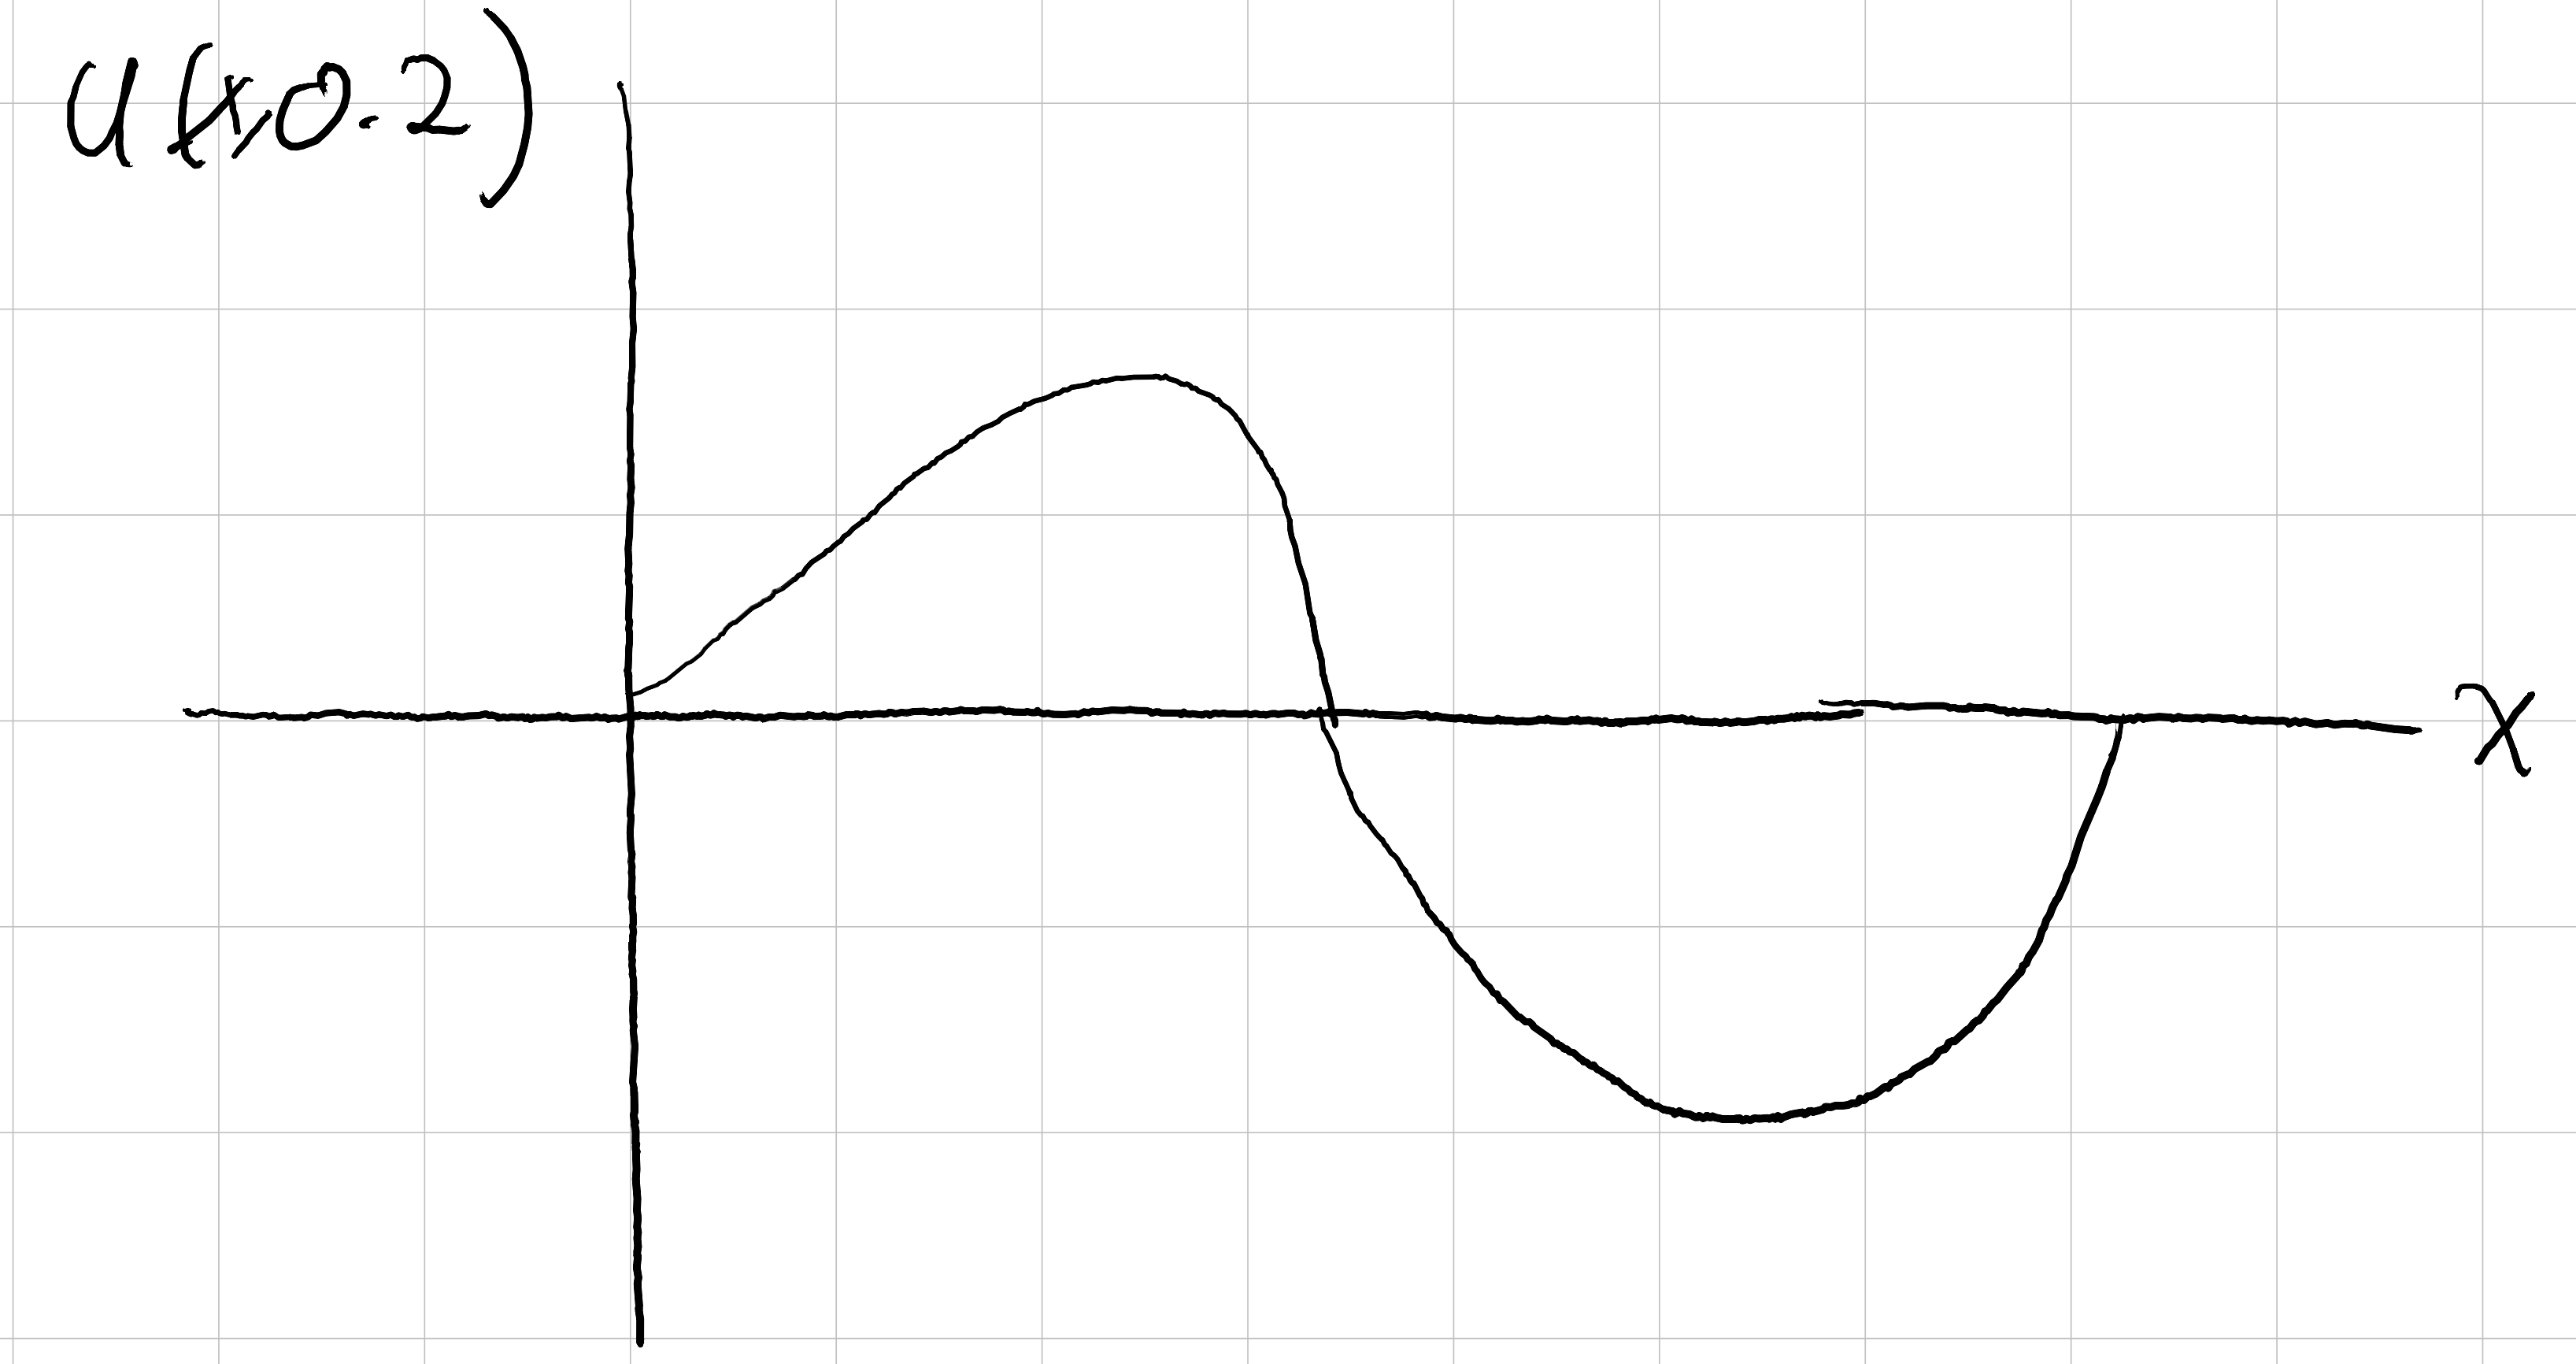
\includegraphics[width=10cm]{images/hw_9_solution_curve_1.png}
  \end{center}
  The solution curve is implicitly defined as
  \begin{align*}
    u\left( x,t \right) &= \sin\left( x-u^2 t \right).
  \end{align*}
\end{solution}
\begin{solution}
  We may write the equation as
  \begin{align*}
    0 &= \pd{u}{t} + \pd{}{x}\left( \frac{1}{4}u^4 \right).
  \end{align*}
  In the sketch below, we see that the wave front moves forward in $x$ as time moves forward if $u$ is positive, and moves backward in $x$ if $u$ is negative, eventually forming a shock. This follows from the fact that one of the characteristic curves is $x_0 = x-u^3 t$.
  \begin{center}
    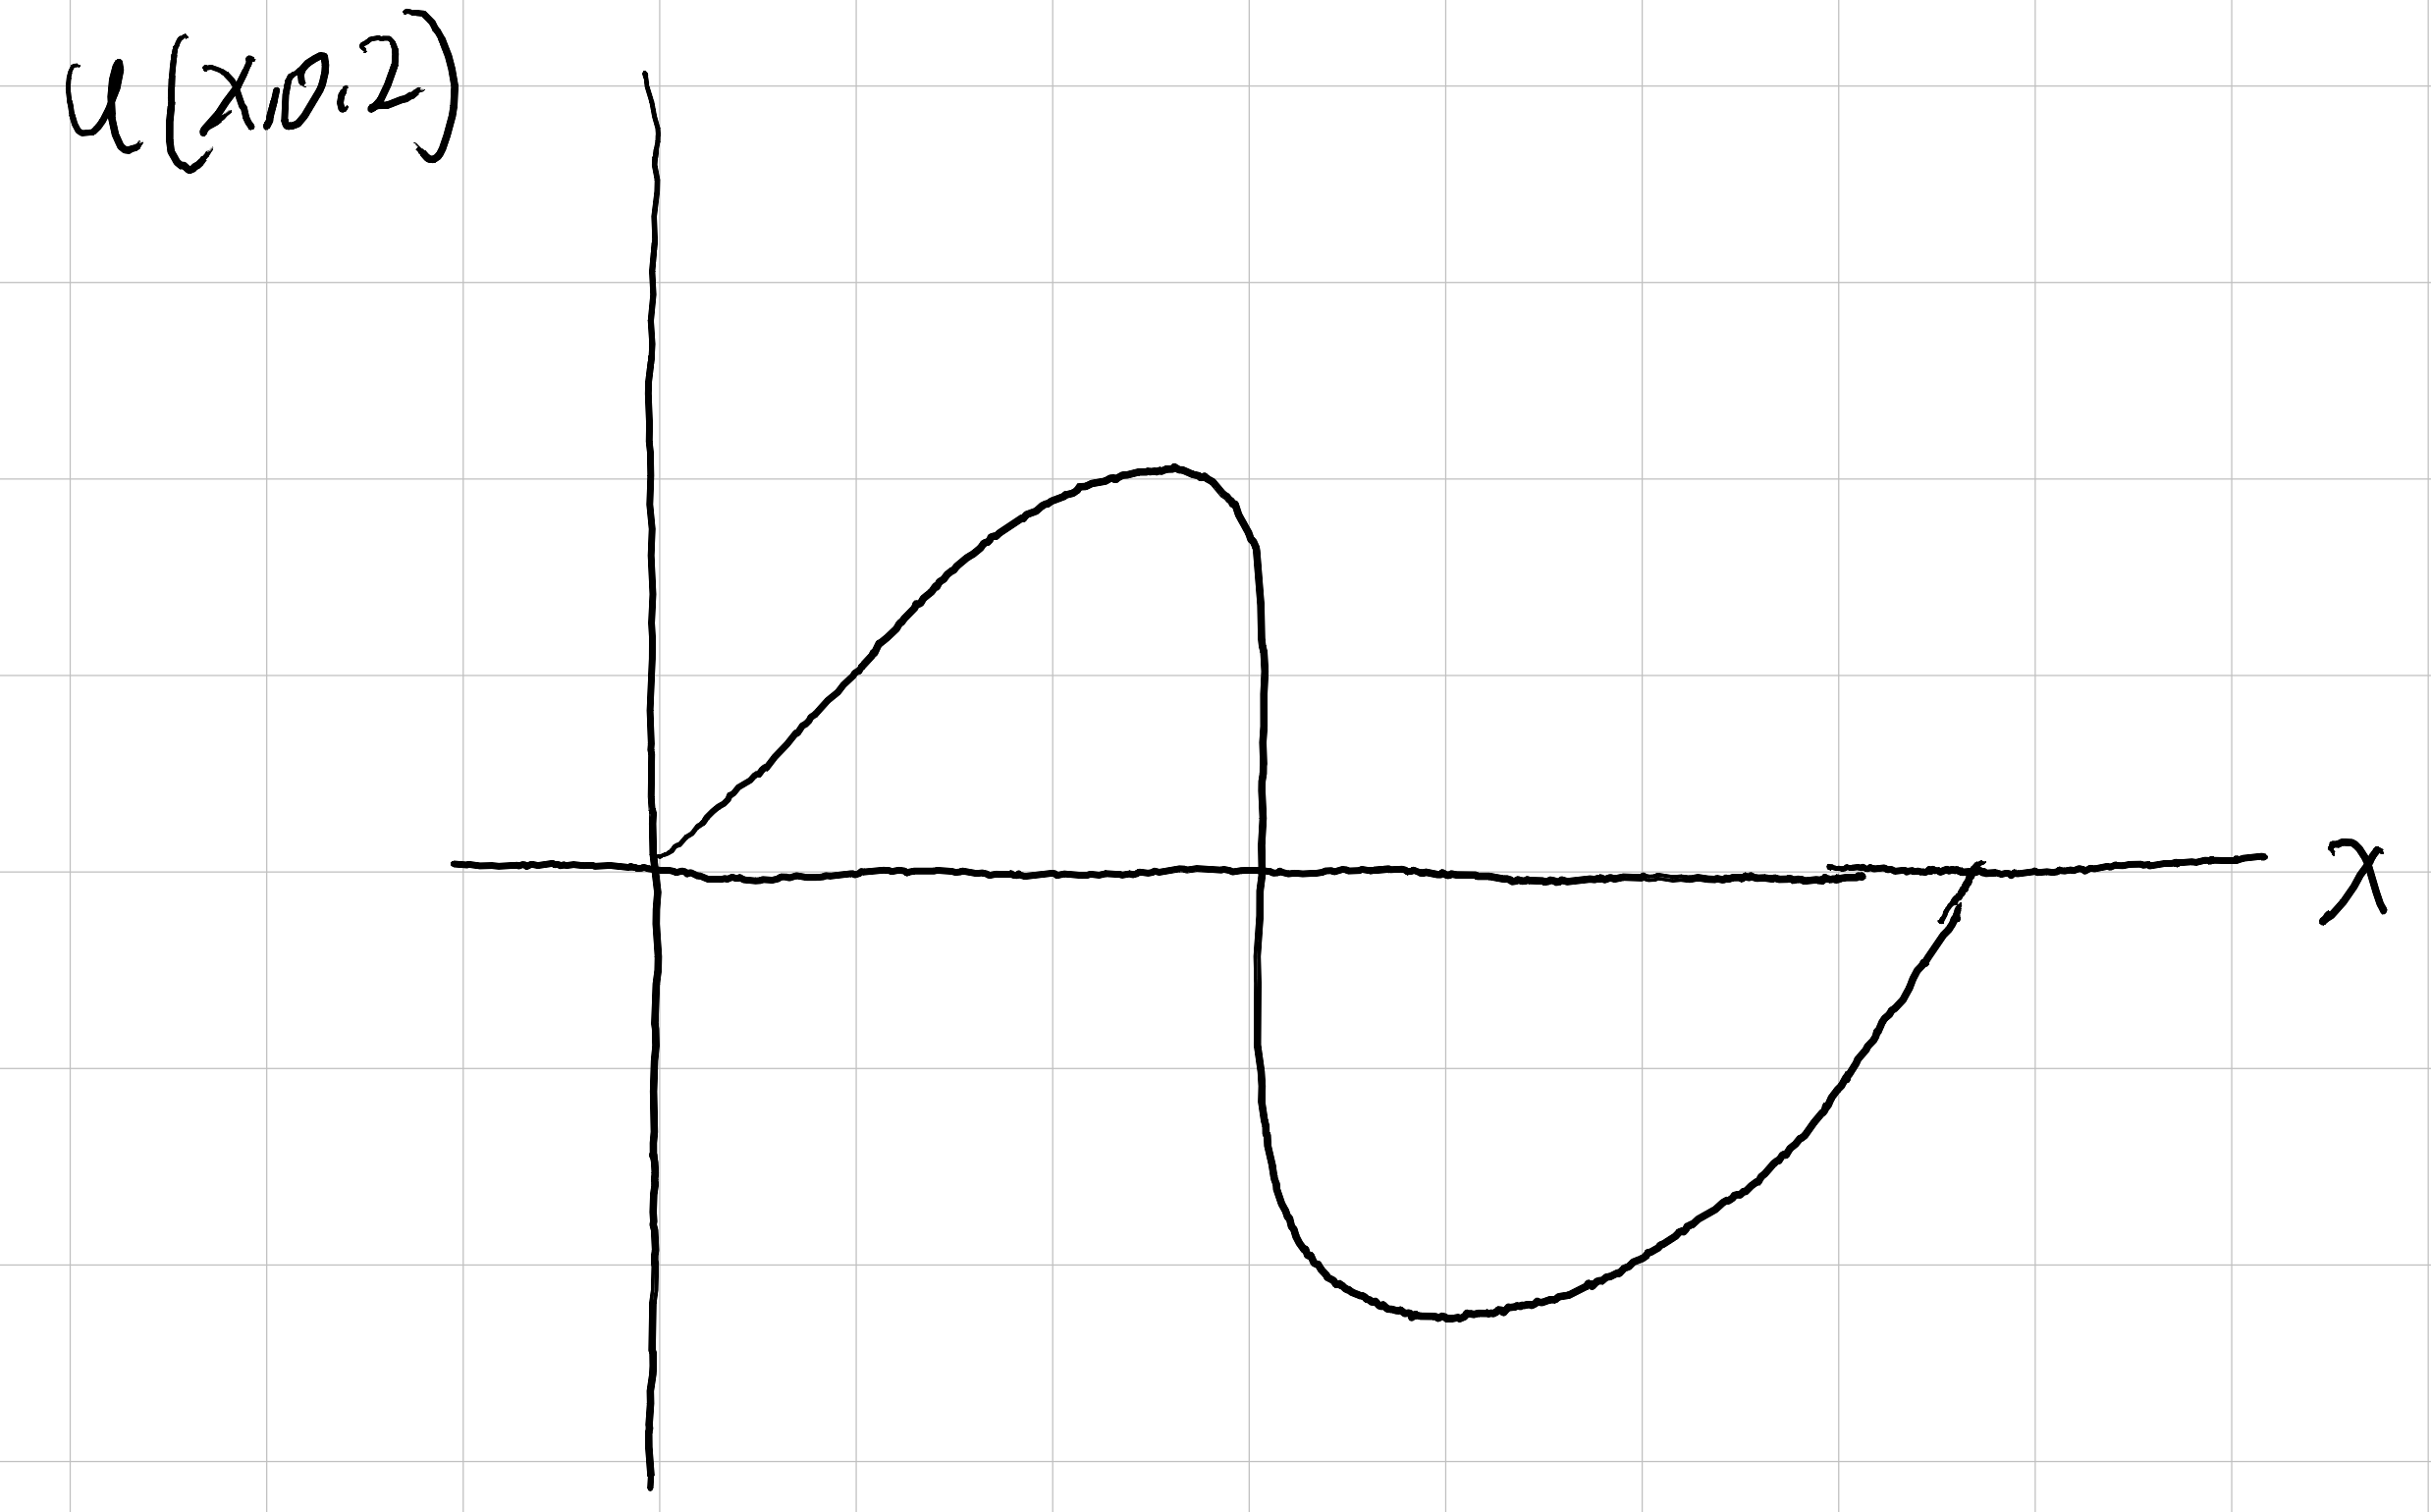
\includegraphics[width=10cm]{images/hw_9_solution_curve_2.png}
  \end{center}
  The solution curve is implicitly defined as
  \begin{align*}
    u\left( x,t \right) &= \sin\left( x-u^3 t \right).
  \end{align*}
  
\end{solution}

\end{document}
